\section{Auswertung}
\label{sec:Auswertung}

\subsection{Strom-Spannungs-Kennlinie für die violette Linie}

In der linken Tabelle von \ref{tab:violett} ist die gemessene Stromstärke von der blauen Linie $I_{v1}$ in Abhängigkeit zur eingestellten Spannung $U$ aufgetragen.
Rechts werden die Werte für die gleiche Messreihe mit der Hälfte der Intensität der ersten Messreihe aufgelistet.

\begin{table}[H]
  \centering
  \caption{Eingetragen ist links die gemessene Stromstärke der blauen Linie abhängig von der eingestellten Spannung. Rechts ist die gleiche Messreihe mit halber Intensität aufgeführt.}
  \label{tab:violett}
  \sisetup{table-format=1.1, per-mode=reciprocal}
  \begin{minipage}[t]{0.2\textwidth}
  \begin{adjustwidth}{}{} 
   \begin{tblr}[t]{
      colspec = {S[table-format=3.2] S[table-format=2.3]},
      row{1} = {guard, mode=math},
    }
    \toprule
    U \mathbin{/} \unit{\volt} & I_{b1} \mathbin{/} \unit{\nano\ampere} \\
    \midrule
    0.98   &   0.000 \\
    0.93   &   0.002 \\
    0.88   &   0.012 \\
    0.83   &   0.030 \\
    0.78   &   0.054 \\
    0.73   &   0.096 \\
    0.68   &   0.170 \\
    0.63   &   0.200 \\
    0.58   &   0.250 \\
    0.53   &   0.370 \\
    0.48   &   0.420 \\
    -0.02   &   1.560 \\
    -0.52   &   4.200 \\
    -1,02   &   7.000 \\
    -1.52   &  11.000 \\
    -2.02   &  15.000 \\
    \bottomrule
  \end{tblr}
\end{adjustwidth}{}{}
\end{minipage}
\hfill
\begin{minipage}[t]{0.2\textwidth} 
 \begin{adjustwidth}{}{} 
   \begin{tblr}[t]{
     colspec = {S[table-format=3.2] S[table-format=2.1]},
     row{1} = {guard, mode=math},
   }
   \toprule
    U \mathbin{/} \unit{\volt} & I_{b1} \mathbin{/} \unit{\nano\ampere} \\
    \midrule
    -3.02   &  25.000 \\
    -4.02   &  32.000 \\
    -5.02   &  36.000 \\
    -6.02   &  40.000 \\
    -7.02   &  44.000 \\
    -8.02   &  48.000 \\
    -9.02   &  50.000 \\
    -10.02   &  52.000 \\
    -11.02   &  52.000 \\
    -12.02   &  54.000 \\
    -13.02   &  54.000 \\
    -14.02   &  56.000 \\
    -15.02   &  56.000 \\
    -16.02   &  56.000 \\
    -17.02   &  58.000 \\
    -18.02   &  58.000 \\
    \bottomrule
   \end{tblr}
 \end{adjustwidth}{}{}
\end{minipage}
\hfill
\begin{minipage}[t]{0.2\textwidth} 
  \begin{adjustwidth}{}{} 
    \begin{tblr}[t]{
      colspec = {S[table-format=3.2] S[table-format=2.1]},
      row{1} = {guard, mode=math},
    }
    \toprule
    U \mathbin{/} \unit{\volt} & I_{b2} \mathbin{/} \unit{\nano\ampere} \\
    \midrule
     0.98 &  0.0\\
    -0.02 &  0.8\\
    -1.02 &  3.2\\
    -2.02 &  6.8\\
    -3.02 & 12.5\\
    -4.02 & 15.0\\
    -5.02 & 17.5\\
    -6.02 & 20.0\\
    -7.02 & 22.5\\
    -8.02 & 25.0\\
    -9.02 & 26.5\\
   -10.02 & 27.5\\
   -11.02 & 27.5\\
   -12.02 & 28.5\\
   -13.02 & 30.0\\
   -14.02 & 28.0\\
   -15.02 & 29.0\\
   -16.02 & 30.0\\
   -17.02 & 30.0\\
   -18.02 & 28.0\\
      \bottomrule
    \end{tblr}
  \end{adjustwidth}{}{}
\end{minipage}
\end{table}

In Abbildung \ref{fig:blau} wird die Stromstärke gegen die Spannung für beide Messreihen aufgetragen.

\begin{figure}[H]
  \centering
  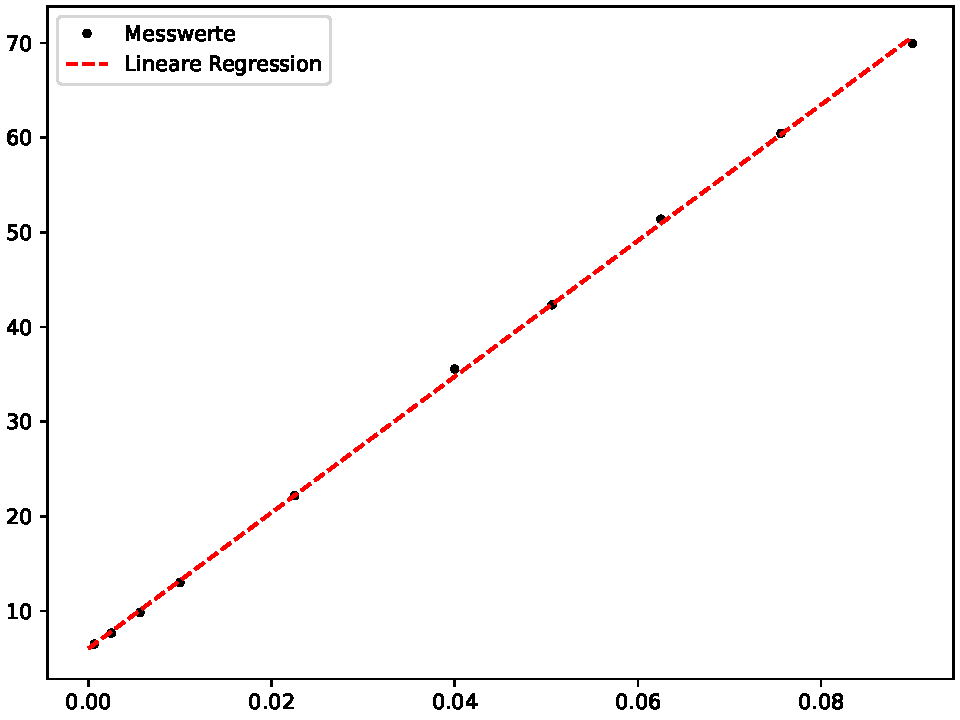
\includegraphics[width=\textwidth]{plot.pdf}
  \caption{Aufgetragen ist die Kennlinie der blauen Linie.}
  \label{fig:blau}
\end{figure}

\subsection{Bestimmung der Grenzspannung}


Die Messwerte für die Stromstärken der violetten, grünen und orangenen Linie sind abhängig von der Spannung in Tabelle \ref{tab:Farben}, in der Reihenfolge von links nach rechts, eingetragen.
\begin{table}[H]
  \centering
  \caption{Aufgeführt ist die Stromstärke in Abhängigkeit zur Spannung. Links ist die Messreihe der violetten Linie, in der Mitte die der Grünen, und rechts die der Orangenen.}
  \label{tab:Farben}
  %\sisetup{table-format=3.1, per-mode=reciprocal}
   \begin{minipage}[t]{0.2\linewidth}
    \begin{tblr}[t]{
        colspec = {S[table-format=1.2] S[table-format=1.3]},
        row{1} = {guard, mode=math},
      }
      \toprule
      U \mathbin{/} \unit{\volt} & I_v \mathbin{/} \unit{\nano\ampere} \\
      \midrule
      1.13  &  0.000 \\
      1.08  &  0.002 \\
      1.03  &  0.006 \\
      0.98  &  0.010 \\
      0.93  &  0.016 \\
      0.88  &  0.026 \\
      0.83  &  0.038 \\
      0.78  &  0.052 \\
      0.73  &  0.062 \\
      0.68  &  0.090 \\
      0.63  &  0.110 \\
      \bottomrule
    \end{tblr}
  \end{minipage}
  \hfill
  \begin{minipage}[t]{0.2\linewidth} 
    \begin{tblr}[t]{
        colspec = {S[table-format=2.2] S[table-format=1.3]},
        row{1} = {guard, mode=math},
      }
      \toprule
      U \mathbin{/} \unit{\volt} & I_g \mathbin{/} \unit{\nano\ampere} \\
      \midrule
      0.45 &  0.000\\
      0.40 &  0.002\\
      0.35 &  0.002\\
      0.30 &  0.004\\
      0.25 &  0.008\\
      0.20 &  0.014\\
      0.15 &  0.020\\
      0.10 &  0.028\\
      0.05 &  0.038\\
      0.00 &  0.048\\
     -0.05 &  0.058\\
      \bottomrule
    \end{tblr}
  \end{minipage}
  \hfill
  \begin{minipage}[t]{0.2\linewidth} 
    \begin{tblr}[t]{
        colspec = {S[table-format=2.2] S[table-format=1.3]},
        row{1} = {guard, mode=math},
      }
      \toprule
      U \mathbin{/} \unit{\volt} & I_o \mathbin{/} \unit{\nano\ampere} \\
      \midrule
      0.25  & 0.000\\
      0.20  & 0.002\\
      0.15  & 0.002\\
      0.10  & 0.004\\
      0.05  & 0.006\\
      0.00  & 0.008\\
     -0.05  & 0.014\\
     -0.10  & 0.016\\
     -0.15  & 0.020\\
     -0.20  & 0.028\\
     -0.25  & 0.036\\
      \bottomrule
    \end{tblr}
  \end{minipage}
  \hfill
\end{table}


Um die Grenzspannung zu bestimmen, wird die Wurzel der Stromstärke von den Farben Violett, Blau, Grün und Orange gegen die eingestellte Spannung aufgetragen.
Dies wird in Abbildung \ref{fig:Farben} dargestellt.
Jetzt kann eine Funktion für die Abhängigkeit der Wurzel der Stromstärke zur Spannung mit linearer Regression erstellt.

\begin{figure}[H]
  \centering
  \includegraphics[width=\textwidth]{Ugrenz.pdf}
  \caption{Abgebildet ist die Abhängigkeit von der Wurzel der Stromnstärke zur Spannung bei den vier gemessenen Linien. 
  Dazu wurde jeweils eine Ausgleichsgerade eingefügt.}
  \label{fig:Farben}
\end{figure}


Damit ergeben sich die Grenzspannungen
\begin{gather*}
  U_{G_v}=\qty{1.138(0.031)}{\volt}\\
  U_{G_b}=\qty{0.966(0.029)}{\volt}\\
  U_{G_g}=\qty{0.453(0.017)}{\volt}\\
  U_{G_o}=\qty{0.280(0.014)}{\volt}.
\end{gather*}

\subsection{Bestimmung der Planck-Konstante}
Für die Bestimmung der Planck-Konstante werden einmal in \ref{fig:Planck} die gemessenen, und einmal die berechneten Grenzspannungen gegen die Frequenz aufgetragen.
Dabei sind die verwendeten Werte für die Frequenzen die, die mit Formel \ref{eqn:Frequenz} und den aus aus Abbildung \ref{fig:Wellenlängen} entnommenen Wellenlängen für Quecksilber berechnet werden.

\begin{figure}[H]
  \centering
  \includegraphics[width=\textwidth]{Planck.pdf}
  \caption{Aufgezeichnet ist links die gemessene Grenzspannung und rechts die Berechnete der verschiedenen Farben in Abhängigkeit zur Frequenz der Linie der Quecksilberdampflampe.
  Zudem wurde eine Ausgleichsgerade hinzugefügt.}
  \label{fig:Planck}
\end{figure}

\begin{figure}[H]
  \centering
  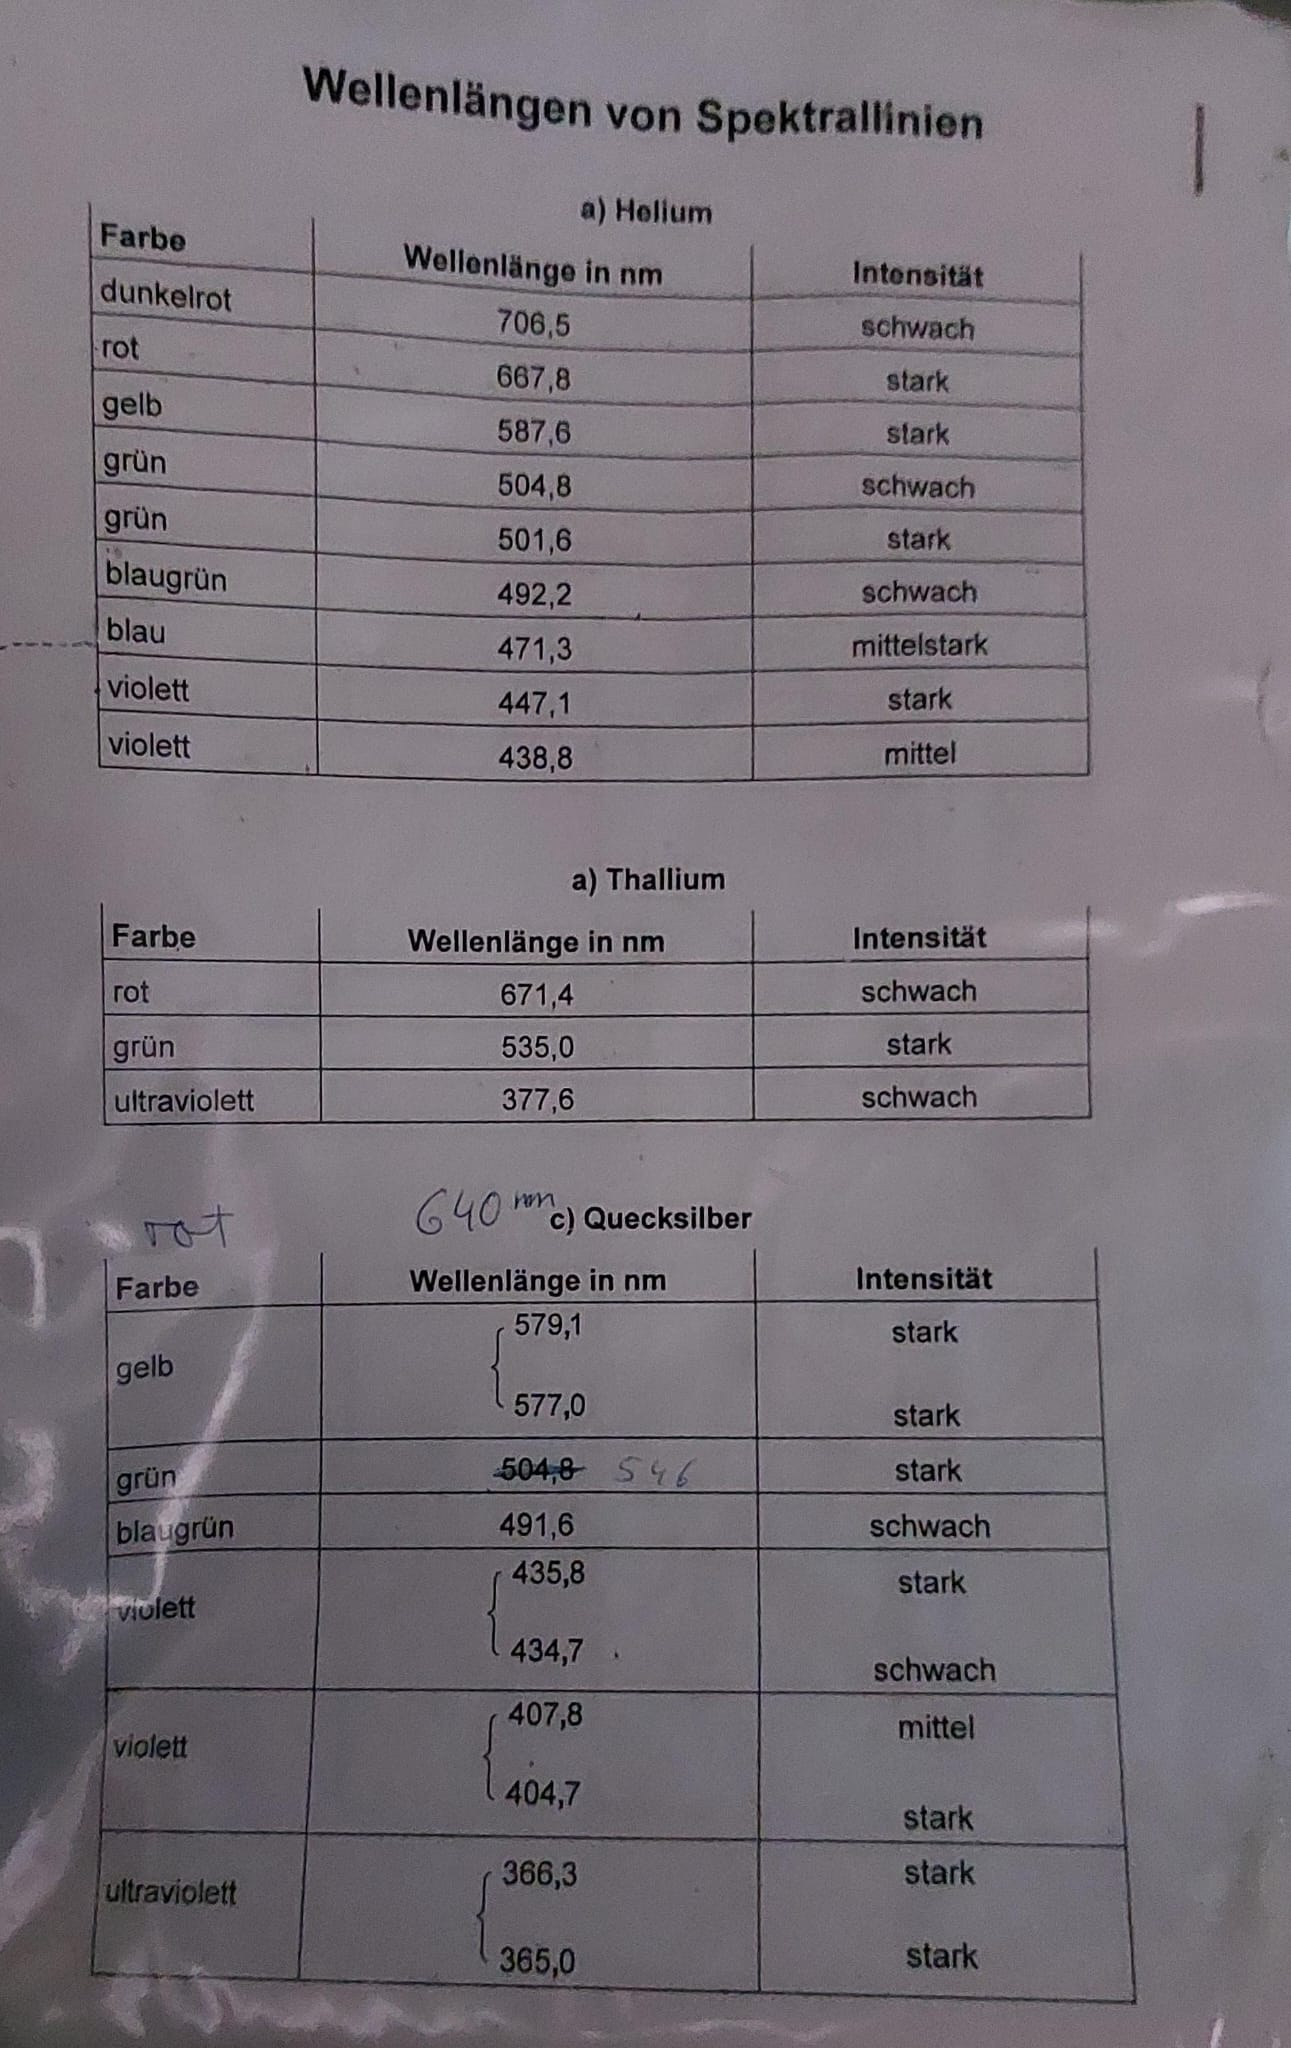
\includegraphics[width=6cm]{Bilder/Well.jpg}
  \caption{Angeführt ist eine Tabelle mit Wellenlängen der Linien verschiedener Lampen.}
  \label{fig:Wellenlängen}
\end{figure}

Die Steigungen der Ausgleichsgeraden entsprechen der Planck-Konstante mit
\begin{gather*}
h_1=\qty{3.860(0.223)e-15}{\electronvolt\second}\\
h_2=\qty{3.886(0.257)e-15}{\electronvolt\second}.
\end{gather*}
Durch Division mit der Elementarladung wird dann 
\begin{gather*}
  h_1=\qty{6.176(0.357)e-34}{\joule\second}\\
  h_2=\qty{6.217(0.411)e-34}{\joule\second}.
\end{gather*}
berechnet.

\subsection{Berechnung der Austrittsarbeit}
Die Austrittsarbeit wird berechnet, indem die Werte für die einzelnen Linien, sowie die nun berechnete Plank-Konstante, in Formel \ref{eqn:hquer} nach $\phi$ umgestellt wird.
Damit ergibt sich 
\begin{gather*}
  \phi_v=\qty{2.76(0.27)e-19}{\electronvolt}\\
  \phi_b=\qty{2.71(0.25)e-19}{\electronvolt}\\
  \phi_g=\qty{2.67(0.20)e-19}{\electronvolt}\\
  \phi_o=\qty{2.75(0.19)e-19}{\electronvolt}
\end{gather*}
mit einem Mittelwert, berechnet mit
\begin{equation}
     \bar{x}=\frac{\sum_{i=1}^{\symup{n}} x_i}{\symup{n}}
     \label{eqn:MW}
\end{equation}
von $\bar{\phi}=\qty{2.72(0.11)e-19}{\electronvolt}$.
